\documentclass[a4paper,14pt]{extarticle}
\usepackage{../../tex-shared/report-layout}

\renewcommand{\mylabnumber}{3}
\renewcommand{\mylabtitle}{Исследование объектной
модели документа (DOM) и системы событий JavaScript}
\renewcommand{\mysubject}{Веб-технологии}
\renewcommand{\mylecturer}{Дрозин А.Ю.}

\begin{document}
\begin{titlepage}
    
    \thispagestyle{empty}
    
    \begin{center}
        
        Министерство науки и Высшего образования Российской Федерации \\
        Севастопольский государственный университет \\
        Кафедра ИС
        
        \vfill

        Отчет \\
        по лабораторной работе №\mylabnumber \\
        \enquote{\mylabtitle} \\
        по дисциплине \\
        \enquote{\MakeTextUppercase{\mysubject}}

    \end{center}

    \vspace{1cm}

    \noindent\hspace{7.5cm} Выполнил студент группы ИС/б-17-2-о \\
    \null\hspace{7.5cm} Горбенко К. Н. \\
    \null\hspace{7.5cm} Проверил \\
    \null\hspace{7.5cm} \mylecturer

    \vfill

    \begin{center}
        Севастополь \\
        \the\year{}
    \end{center}

\end{titlepage}

\section{Цель работы}
Изучить динамическую объектную модель документа, предоставляемую
стандартом DOM и систему событий языка JavaScript, возможность
хранения данных на стороне клиента. Приобрести практические навыки
работы с событиями JavaScript, деревом документа, Local Storage и
Cookies.

\section{Задание на работу}
\begin{enumerate}
    \item Реализовать отображение в области меню сайта текущих даты и
          времени (обновление времени 1 раз в секунду). 
    \item На странице «Контакт» добавить поле «Дата рождения», для
          которого реализовать всплывающий снизу элемент «календарь».
    \item Реализовать динамическую проверку корректности заполнения
          пользователем формы на странице «Контакт» таким образом, чтобы при
          потере фокуса заполняемого поля осуществлялась проверка корректности
          его заполнения. В случае если поле заполнено корректно, оно должно быть
          подсвечено зеленым цветом, иначе оно должно быть подсвечено красным,
          а после данного поля должна появиться надпись, поясняющая характер
          ошибки. После исправления пользователем ошибки, надпись должна исчезнуть. Если все поля формы заполнены корректно должна стать активной кнопка «Отправить».
    \item Реализовать открытие в динамически формируемом новом окне
          (блоке DIV) соответствующих больших фото при щелчке мыши
          по маленьким фото на странице «Фотоальбом».
    \item Добавить страницу «История просмотра». На данной странице
          реализовать отображение двух таблиц: \enquote{История текущего сеанса},
          \enquote{История за все время}.
\end{enumerate}

\section{Ход работы}
\subsection{Дата и время в меню сайта}
Реализуем отображение в меню сайта текущих даты и времени. Для этого добавим модуль следующего содержания:

\begin{lstlisting}
export const formatDate = (date: Date): string => {
    return `${date.getDate()}.` +
            `${date.getMonth() + 1}.` +
            `${date.getFullYear()}, ` +
            `${date.toLocaleString(window.navigator.language, { weekday: 'long'})}`;
};

export const formatTime = (time : Date): string => {
    return time.toLocaleString(window.navigator.language, { hour: '2-digit', minute: '2-digit', second: '2-digit' });
};

const formatCurrentDate = () => {
    return formatDate(new Date());
};

const formatCurrentTime = (): string => {
    return formatTime(new Date());
};

export const updateClockOnInterval = (dateElement: HTMLElement, timeElement: HTMLElement, interval: number) => {
    dateElement.innerHTML = formatCurrentDate();
    timeElement.innerHTML = formatCurrentTime();
    setInterval(() => {
        dateElement.innerHTML = formatCurrentDate();
        timeElement.innerHTML = formatCurrentTime();
    }, interval);
};
\end{lstlisting}

Используется данный модуль следующим образом:

\begin{lstlisting}
import { updateClockOnInterval } from '../clock/clock';

window.onload = () => {
    updateClockOnInterval(document.getElementById('date'), document.getElementById('time'), 1000);
};
\end{lstlisting}

Добавим в HTML разметку новые элементы:

\begin{lstlisting}
<nav>
    <ul>
        <li><span                   >Web lab1</span></li>
        <li><a href="index.html"    >Home</a></li>
        <li><a href="about.html"    >About</a></li>
        <li><a href="interests.html">My interests</a></li>
        <li><a href="learning.html" >Learning</a></li>
        <li><a href="photos.html"   >Photos</a></li>
        <li><a href="contact.html"  >Contact</a></li>
        <li><a href="test.html"     >Test</a></li>
        <li><a href="history.html"  >History</a></li>
        <li><span id="time"></span><br><span id="date"></span></li>
    </ul>
</nav>
\end{lstlisting}

Результат изображен на рисунке \ref{fig:clock}:

\begin{figure}[H]
    \centering
    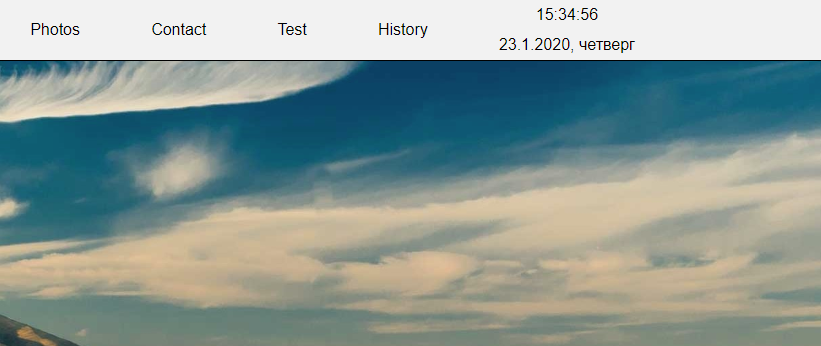
\includegraphics[width=.8\linewidth]{clock}
    \caption{Дата и время в меню сайта}
    \label{fig:clock}
\end{figure}

\subsection{Мои интересы}
На странице \enquote{Мои интересы} реализуем выведение содержания по нажатию на
соответствующий пункт меню:

\begin{lstlisting}
enum InterestIds {
    Hobbies = 'Hobbies', 
    Books   = 'Books', 
    Music   = 'Music', 
    Films   = 'Films'
}

type InterestsNode = {
    [key in keyof typeof InterestIds]: InterestsNodeContent
}

interface InterestsNodeContent {
    header: string;
    values: string[];
    isHidden: boolean;
}

window.onload = () => {
    updateClockOnInterval(document.getElementById('date'), document.getElementById('time'), 1000);
    let interestsLinks = document.getElementsByClassName('contents');

    Array.from(interestsLinks).forEach(link => {
        link.addEventListener('click', handleClick);
    });
};

const handleClick = (event) : void => {
    const target = event.target as HTMLElement;
    if (interests[target.id].isHidden) {
        insertAfter(createInterestNode(target.id), target);
        interests[target.id].isHidden = false;
    } else {
        removeElementById(`${target.id}-expand`);
        interests[target.id].isHidden = true;
    }
};

const createInterestNode = (interestId: string) => {
    const interestContent = interests[interestId];
    const interestNode = createElement('li', { id: `${interestId}-expand`, classList: ['interests'] });
    appendChildren(interestNode,
        createElement('h2', { innerHTML: interestContent.header }),
        createElement('p', { innerHTML: interestContent.values[0] }),
        createElement('p', { innerHTML: interestContent.values[1] })
    );
    return interestNode;
};
\end{lstlisting}

Обновим HTML документ:

\begin{lstlisting}
<section>
<header><h2>Contents</h1></header>
<ul id="interests">
    <li class="contents" id="Hobbies">Мои хобби.</li>
    <li class="contents" id="Books">Мои книги.</li>
    <li class="contents" id="Music">Моя музыка.</li>
    <li class="contents" id="Films">Мои фильмы.</li>
</ul>
</section>
\end{lstlisting}

Меню выглядит следующим образом (рисунок \ref{fig:interests}):

\begin{figure}[H]
    \centering
    \subfloat[До нажатия]{
\includegraphics[width=.4\linewidth]{before}}
    \hspace{.15\linewidth}
    \subfloat[После нажатия]{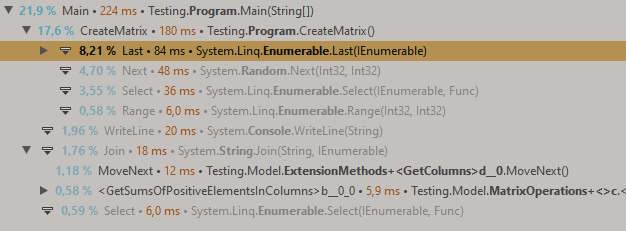
\includegraphics[width=.4\linewidth]{after}}
    \caption{Выпадающее меню на странице \enquote{Мои интересы}}
    \label{fig:interests}
\end{figure}

\subsection{Формы}
\subsubsection{Выбор даты}

Для реализации выбора даты создадим отдельный модуль. Его содержание:

\begin{lstlisting}
import { createElementWithClass, createElementWithInnerHTML, createElementWithId } from '../utils/dom';
import { formatDate } from '../clock/clock';

const datepickerId = 'datepicker';
const datepickerInputId = 'datepicker-input';
const datepickerYearSelectId = 'datepicker-year';
const datepickerMonthSelectId = 'datepicker-month';
const datepickerDateListId = 'datepicker-date-list';
const elementWrapperClass = 'element-wrapper';

const datepicker = () => document.querySelector('#' + datepickerId);
const datepickerInput = () => document.querySelector('#' + datepickerInputId);
const yearSelect = () => document.querySelector('#' + datepickerYearSelectId);
const monthSelect = () => document.querySelector('#' + datepickerMonthSelectId);
const dateList = () => document.querySelector('#' + datepickerDateListId);

let selectedYear, selectedMonthNumber, selectedDate;
let isShown = false;

export default () => {
    datepickerInput().addEventListener('click', showDatePicker);
    window.addEventListener('click', (event) => removeDatePicker(event));
}

const insertDate = (event) => {
    if (event.target !== dateList()) {
        selectedYear = (yearSelect() as HTMLFormElement).value;
        selectedMonthNumber = months.indexOf((monthSelect() as HTMLFormElement).value);
        selectedDate = event.target.innerHTML;
        const date = new Date(selectedYear, selectedMonthNumber, selectedDate);

        (datepickerInput() as HTMLElement).focus();
        (datepickerInput() as HTMLFormElement).value = formatDate(date);
        (datepickerInput() as HTMLElement).blur();
    }
};

const showDatePicker = () => {
    if (!isShown) {
        datepickerInput().parentNode.insertBefore(createDatePicker(), datepickerInput().nextSibling);
        Array.from(dateList().childNodes).forEach(listItem => {
            listItem.addEventListener('click', (event) => insertDate(event));
        });
        yearSelect().addEventListener('change', updateDatesList);
        monthSelect().addEventListener('change', updateDatesList);
        isShown = true;
    }
};

const removeDatePicker = (event) => {
    if (isShown && !datepicker().contains(event.target as Node) && event.target !== datepickerInput()) {
        (datepickerInput() as HTMLElement).blur();
        datepicker().remove();
        isShown = false;
    }
};

const createDatePicker = () => {
    const date = new Date();
    let datepicker = createElementWithId('div', datepickerId);
    let yearAndMonthSelectsWrapper = createElementWithClass('div', elementWrapperClass);
    let dateListWrapper = createElementWithClass('div', elementWrapperClass);
    yearAndMonthSelectsWrapper.appendChild(createYearsSelect());
    yearAndMonthSelectsWrapper.appendChild(createMonthSelect());
    datepicker.appendChild(yearAndMonthSelectsWrapper);
    dateListWrapper.appendChild(createDatesList(selectedYear || date.getFullYear(), selectedMonthNumber + 1 || date.getMonth() - 1));
    datepicker.appendChild(dateListWrapper);

    return datepicker;
};

const updateDatesList = () => {
    const selectedYear = (yearSelect() as HTMLFormElement).value;
    const selectedMonthNumber = months.indexOf((monthSelect() as HTMLFormElement).value);
    const dateListWrapper = dateList().parentElement;

    dateList().remove();
    const newDateList = createDatesList(selectedYear, selectedMonthNumber + 1);
    newDateList.addEventListener('click', (event) => insertDate(event));
    dateListWrapper.appendChild(newDateList);
};

const createYearsSelect = () => {
    const selectYear = createElementWithId('select', datepickerYearSelectId);
    getYears().forEach(year => {
        selectYear.appendChild(createElementWithInnerHTML('option', year));
    });
    (selectYear as HTMLFormElement).value = selectedYear || new Date().getFullYear();
    return selectYear;
};

const createMonthSelect = () => {
    const selectMonth = createElementWithId('select', datepickerMonthSelectId);
    months.forEach(month => {
        selectMonth.appendChild(createElementWithInnerHTML('option', month));
    });
    (selectMonth as HTMLFormElement).value = months[selectedMonthNumber] || months[new Date().getMonth()];
    return selectMonth;
};

const createDatesList = (year, month) => {
    let dateList = createElementWithId('ul', datepickerDateListId);
    getDays(getNumberOfDaysInMonth(year, month)).forEach(date => {
        dateList.appendChild(createElementWithInnerHTML('li', date));
    });
    return dateList;
};

const getNumberOfDaysInMonth = (year, month) => {
    return new Date(year, month, 0).getDate();
};

const getYears = () => {
    let years = [];
    for (let i = 2000; i <= 2025; i++) {
        years.push(i);
    }
    return years;
};

const getDays = (n : number) => {
    let days = [];
    for (let i = 1; i <= n; i++) {
        days.push(i);
    }
    return days;
};

const months = ['January', 'February', 'March', 'April', 'May', 'June', 'July', 'August', 'September', 'October', 'November', 'December'];
\end{lstlisting}

Используем этот элемент:
\begin{lstlisting}
<li>
    <label for="datepicker-input">Date</label>
    <input type="text" name="date" id="datepicker-input" class="field-long" />
</li>
\end{lstlisting}

Настроим валидацию для этого элемента:
\begin{lstlisting}
import { FormComponent, NameValidator, FieldFilledValidator, PhoneNumberValidator, setFieldsForValidation, DateValidator } from '../forms/forms';

window.onload = () => {
    datepicker();
    setFieldsForValidation(fields, document.forms.item(0));
};

const fields: FormComponent[] = [
    ...
    new FormComponent(
        'datepicker-input',
        [
            new DateValidator()
        ]
    )
];
\end{lstlisting}

Класс \code{DateValidator} из модуля \code{forms}:
\begin{lstlisting}
export class DateValidator implements FormValidator {
    errorMessage = 'Date was not in correct format';
    validate = (value: string) : Boolean => {
        const pattern = /^\d{1,2}\.\d{1,2}\.\d{4}, [а-яА-Я]+$/;
        return pattern.test(value);
    };
}
\end{lstlisting}

Элемент изображен на рисунке \ref{fig:datepicker}.

\begin{figure}[H]
    \centering
    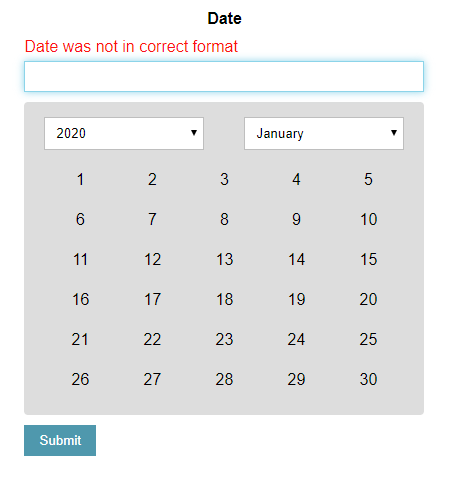
\includegraphics[width=.4\linewidth]{datepicker}
    \caption{Элемент для выбора даты и времени}
    \label{fig:datepicker}
\end{figure}

\subsection{Просмотр фотографий}
Реализуем просмотр фотографий по нажатию. Логика реализована в соответствующем модуле.

\begin{lstlisting}
import { createElement } from '../utils/dom'

const lightboxId = 'lightbox';
const lightboxClass = 'lightbox';
const lightboxPictureClass = 'lightbox-picture';
const lightboxCloseButtonClass = 'lightbox-close';

export default (lightboxPhotosWrapper: Element) => {
    lightboxPhotosWrapper.addEventListener('click', (event) => expandLightbox(event));

    window.onclick = (event) => {
        if (event.target === document.getElementById(lightboxId)) {
            collapseLightbox();
        }
    }
}

const expandLightbox = (event) => {
    const lightbox = createElement('div', { id: lightboxId, classList: [lightboxClass] });
    const image = createElement('img', { src: event.target.src, classList: [lightboxPictureClass] });
    const closeButton = createElement('div', { innerHTML: '&times', classList: [lightboxCloseButtonClass], onclick: () => collapseLightbox() });

    lightbox.appendChild(image);
    lightbox.appendChild(closeButton);
    document.body.appendChild(lightbox);
};

const collapseLightbox = () => {
    const lightbox = document.getElementById(lightboxId);
    lightbox.remove();
};
\end{lstlisting}

Использование модуля:

\begin{lstlisting}
import addLightbox from '../lightbox/lightbox';

window.onload = () => {
    let photoWrapper = document.querySelector('.photo-wrapper');
    addLightbox(photoWrapper);
};
\end{lstlisting}

Элемент изображен на рисунке \ref{fig:lightbox}.

\begin{figure}[H]
    \centering
    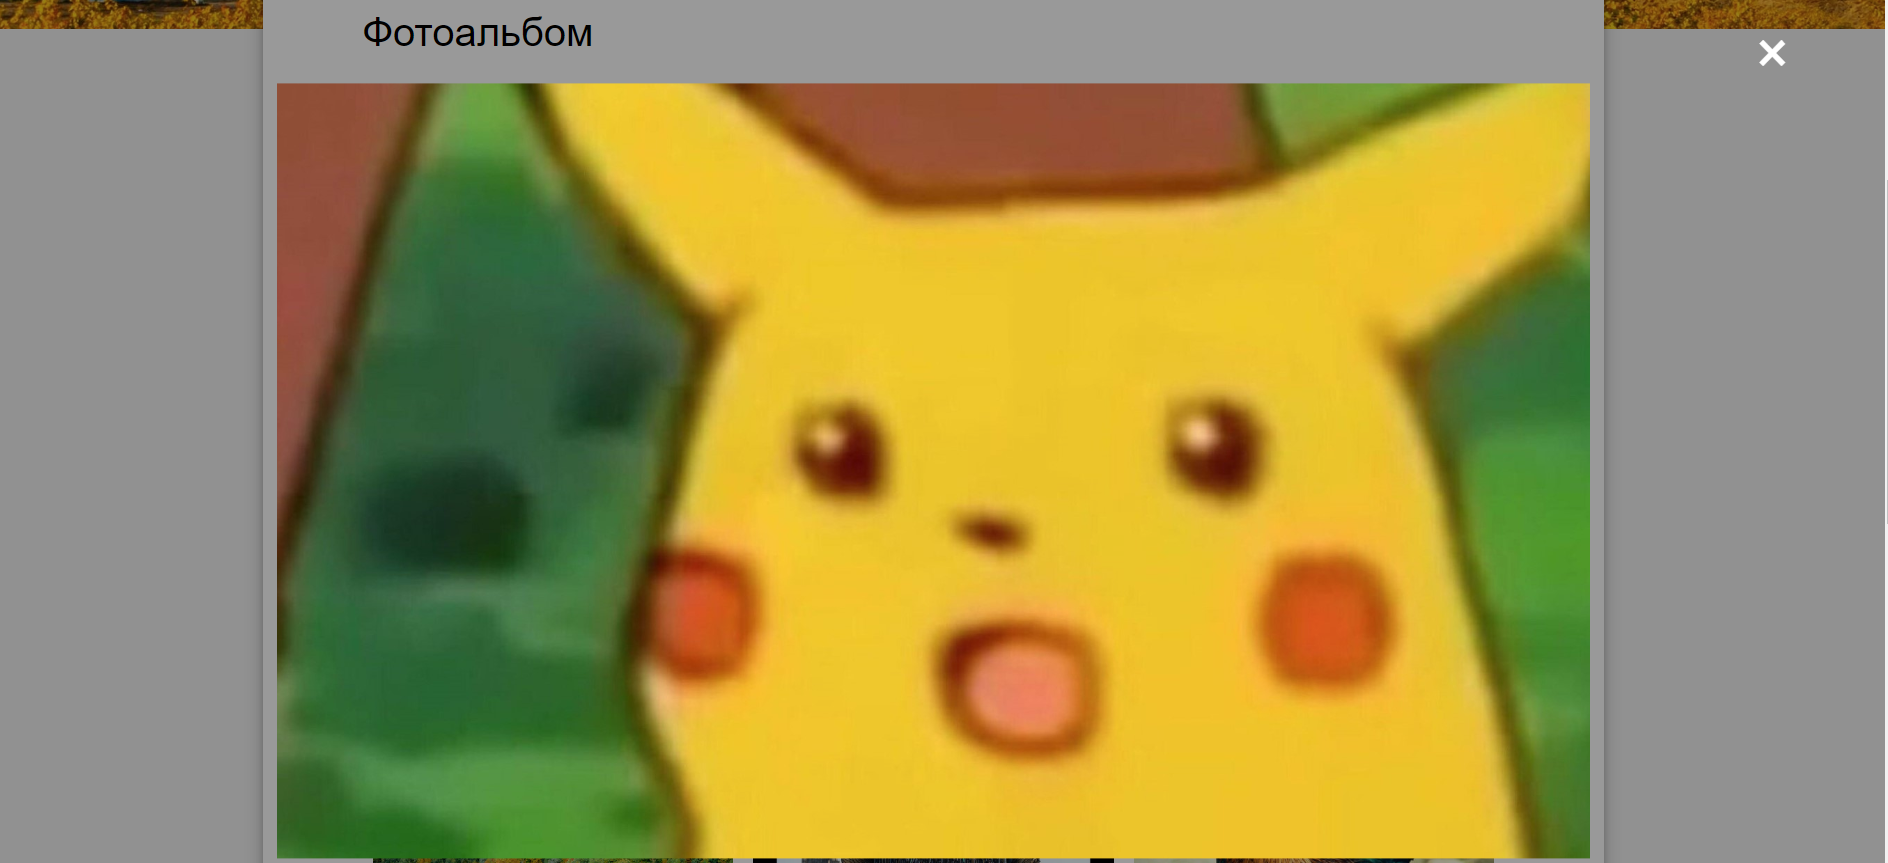
\includegraphics[width=.8\linewidth]{lightbox}
    \caption{Элемент для выбора даты и времени}
    \label{fig:lightbox}
\end{figure}

\subsection{История просмотра}
Реализация истории просмотра в отдельном модуле:

\begin{lstlisting}
type Pages = 'home'
    | 'about'
    | 'interests'
    | 'learning'
    | 'photos'
    | 'contact'
    | 'test'
    | 'history';

type PageHistory = {[key in Pages]: number;};

export const visitPage = (page: Pages) => {
    incrementLocalStoragePageVisits(page);
    incrementSessionStoragePageVisits(page);
};

const incrementLocalStoragePageVisits = (page: Pages) => {
    const currentLocalStorageValue = getLocalStorageValue(page);
    if (currentLocalStorageValue) {
        setLocalStorageValue(page, (Number(currentLocalStorageValue) + 1).toString());
    } else {
        setLocalStorageValue(page, '1');
    }
};

const incrementSessionStoragePageVisits = (page: Pages) => {
    const currentSessionStorageValue = getSessionStorageValue(page);
    if (currentSessionStorageValue) {
        setSessionStorageValue(page, (Number(currentSessionStorageValue) + 1).toString());
    } else {
        setSessionStorageValue(page, '1');
    }
};

export const getGlobalHistory = (): PageHistory => {
    return {
        home: Number(getLocalStorageValue('home')),
        about: Number(getLocalStorageValue('about')),
        interests: Number(getLocalStorageValue('interests')),
        learning: Number(getLocalStorageValue('learning')),
        photos: Number(getLocalStorageValue('photos')),
        contact: Number(getLocalStorageValue('contact')),
        test: Number(getLocalStorageValue('test')),
        history: Number(getLocalStorageValue('history'))
    };
};

export const getSessionHistory = () => {
    return {
        home: Number(getSessionStorageValue('home')),
        about: Number(getSessionStorageValue('about')),
        interests: Number(getSessionStorageValue('interests')),
        learning: Number(getSessionStorageValue('learning')),
        photos: Number(getSessionStorageValue('photos')),
        contact: Number(getSessionStorageValue('contact')),
        test: Number(getSessionStorageValue('test')),
        history: Number(getSessionStorageValue('history'))
    };
};

export const getLocalStorageValue = (name: string) => {
    return localStorage.getItem(name);
};

export const setLocalStorageValue = (name: string, value: string) => {
    localStorage.setItem(name, value);
};

export const getSessionStorageValue = (name: string) => {
    return sessionStorage.getItem(name);
};

export const setSessionStorageValue = (name: string, value: string) => {
    sessionStorage.setItem(name, value);
};
\end{lstlisting}

Поместим на каждую страницу логику сохранения информации о посещених:

\begin{lstlisting}
import { visitPage } from '../storage/storage';

window.onload = () => {
    visitPage('home');
};
\end{lstlisting}

Реализуем страницу истории посещений:
\begin{lstlisting}
<div class="main-content">
    <header><h1>История</h1></header>
    <section>
        <header><h2>История сессии</h2></header>
        <table class="session-history">
            <tr><th colspan="2"> История сессии</th></tr>
            <tr><td>Домашняя страница</td><td class='home'></td></tr>
            <tr><td>Обо мне</td><td class='about'></td></tr>
            <tr><td>Мои интересы</td><td class='interests'></td></tr>
            <tr><td>Учеба</td><td class='learning'></td></tr>
            <tr><td>Фото</td><td class='photos'></td></tr>
            <tr><td>Контакт</td><td class='contact'></td></tr>
            <tr><td>Тест</td><td class='test'></td></tr>
            <tr><td>История</td><td class='history'></td></tr>
        </table>
    </section>
    <section>
        <header><h2>История за все время</h2></header>
        <table class="global-history">
            <tr><th colspan="2">История за все время</th></tr>
            <tr><td>Домашняя страница</td><td class='home'></td></tr>
            <tr><td>Обо мне</td><td class='about'></td></tr>
            <tr><td>Мои интересы</td><td class='interests'></td></tr>
            <tr><td>Учеба</td><td class='learning'></td></tr>
            <tr><td>Фото</td><td class='photos'></td></tr>
            <tr><td>Контакт</td><td class='contact'></td></tr>
            <tr><td>Тест</td><td class='test'></td></tr>
            <tr><td>История</td><td class='history'></td></tr>
        </table>
    </section>
</div>
\end{lstlisting}

\begin{lstlisting}
import { getGlobalHistory, getSessionHistory, visitPage } from '../storage/storage';

window.onload = () => {
    visitPage('history');
    const globalHistory = getGlobalHistory();
    for (let key in globalHistory) {
        const pageHistoryCell = document.querySelector(`.global-history .${key}`);
        pageHistoryCell.innerHTML = globalHistory[key];
    }
    const sessionHistory = getSessionHistory();
    for (let key in sessionHistory) {
        const pageHistoryCell = document.querySelector(`.session-history .${key}`);
        pageHistoryCell.innerHTML = sessionHistory[key];
    }
};
\end{lstlisting}

Страница истории просмотров имеет вид, изображенный на рисунках \ref{fig:session-history} - \ref{fig:global-history}.

\begin{figure}[H]
    \centering
    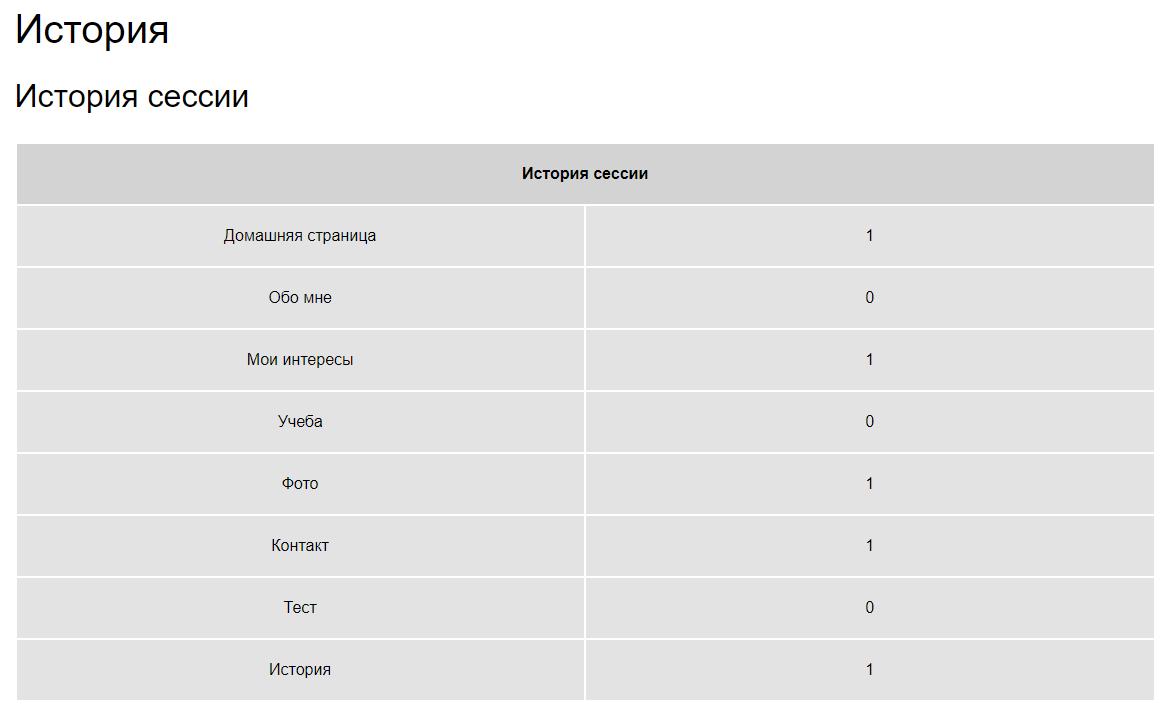
\includegraphics[width=.8\linewidth]{session-history}
    \caption{История сессии}
    \label{fig:session-history}
\end{figure}

\begin{figure}[H]
    \centering
    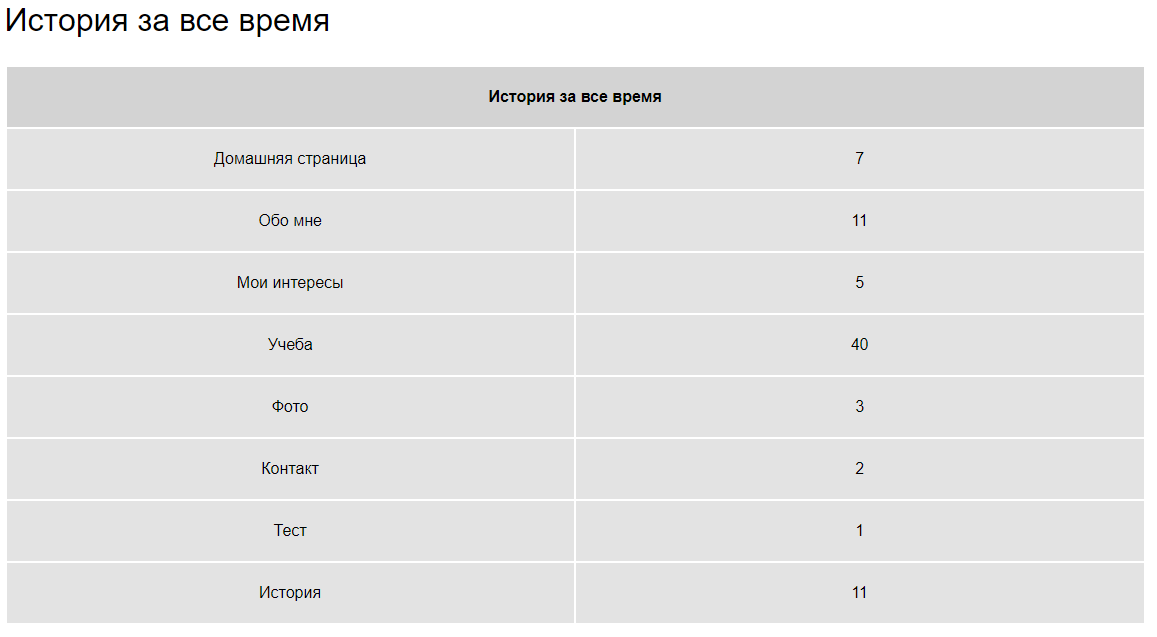
\includegraphics[width=.8\linewidth]{global-history}
    \caption{История за все время}
    \label{fig:global-history}
\end{figure}

\section*{Вывод}
В ходе лабораторной работы активно использовался DOM API. Для получения элементов DOM можно использовать функции
\code{getElementById}, \code{getElementsByClassName}, \code{querySelector}. Для размещения объектов \code{JavaScript}
в DOM используются функции \code{appendChild}, \code{insertBefore}.

Недостатком DOM API является многословность при выполнении даже базовых операций, что приводит к тому, что код сложно
поддерживать. Кроме того, отсутстует поддержка привязки данных к объектам DOM.
\end{document}